\chapter{Método de Trabajo}
\label{chap:metodo}

\drop{E}{n} este capítulo se detalla la metodología utilizada para el desarrollo del presente \ac{TFG} así como las tecnologías utilizadas para llevar a término el proyecto.

Para la gestión y el desarrollo del \ac{TFG} se utilizará Kanban y \ac{TDD}, haciendo uso del desarrollo evolutivo.

Kanban proporciona un método productivo bien delineado en fases que garantiza que el cambio a la siguiente fase no se producirá hasta haberse completado correctamente la fase actual.

El desarrollo del producto software se realizará mediante \ac{TDD}, ya que es una solución que permite asegurarse del correcto funcionamiento de los componentes antes de permitir el siguiente paso.

Mediante el prototipado evolutivo conseguiremos ir perfilando el producto final mediante un acercamiento por fases terminadas.

Por tanto, el prototipado nos marcará la meta de cada fase, kanban nos indicará los objetivos individuales necesarios para alcanzar el final de cada una de las fases y \ac{TDD} nos permitirá asegurarnos que los componentes desarrollados poseen la calidad exigida por kanban para terminar el desarrollo del objetivo individual.


\section{Dispositivos empleados}
Para el desarrollo del \ac{TFG} se utilizarán los siguientes dispositivos:

	\subsection{Ordenador portátil}
	
	Para el desarrollo del TFG se ha utilizado un ordenador portátil con las características que se detallan en la tabla \ref{tab:portatil}.
	
	\begin{table}[H]
	  \centering 
	  \rowcolors{1}{gray!25}{white}
	  \begin{tabular}{p{0.4\linewidth}p{0.3\linewidth}}
	    \toprule
	    Fabricante 							& Acer 											\\
	    Modelo								& Aspire V 15 Nitro								\\
		Fabricante Procesador 				& Intel 										\\
		Modelo Procesador 					& i7-5500U 										\\
		Velocidad y Núcleos del Procesador & 2.4 GHz; 2 núcleos 							\\
		Memoria RAM 						& 16 \ac{GB} \ac{DDR}3L \ac{SDRAM} 			\\
		Disco Duro Principal y Secundario 	& 250 \ac{GB} \ac{SDD} y 1 \ac{TB} \ac{HDD}	\\
		Sistema Operativo					& Elementary \ac{OS} 							\\
	    \hline
	  \end{tabular}
	  \caption{Ordenador utilizado para el desarrollo \ac{TFG}}
	  \label{tab:portatil}
	\end{table}
	
	\subsection{Teléfono móvil}
	
	Para las pruebas del desarrollo en dispositivos móviles se ha utilizado un teléfono móvil con las características que se detallan en la table \ref{tab:movil}.
	
	\begin{table}[H]
	  \centering 
	  \rowcolors{1}{gray!25}{white}
	  \begin{tabular}{p{0.4\linewidth}p{0.3\linewidth}}
	    \toprule
	    Fabricante 				& LG 				\\
	    Modelo 					& D820 (Nexus 5) 	\\
		Fabricante Procesador 	& Qualcomm 			\\
		Modelo Procesador 		& Snapdragon 800 	\\
		Velocidad Procesador 	& 2.26 GHz 			\\
		Memoria RAM 			& 2 \ac{GB} 		\\
		Sistema Operativo 		& Android 6.0 		\\
		Tamaño Pantalla			& 4.95 pulgadas 	\\
	    \hline
	  \end{tabular}
	  \caption{Dispositivo móvil utilizado para el desarrollo \ac{TFG}}
	  \label{tab:movil}
	\end{table}

\section{Desarrollo evolutivo}
También conocido como prototipado evolutivo, este tipo de desarrollo se basa en exponer una implementación inicial al usuario permitiendo, a través de sus comentarios, refinar el sistema mediante versiones hasta alcanzar el producto final.
Este tipo de enfoque es más efectivo que un desarrollo en cascada debido a que satisface las necesidades inmediatas del cliente y debido a que utiliza un enfoque evolutivo, la especificación del producto se desarrolla de forma creciente en tanto en cuanto el cliente comienza a mejorar su comprensión y acercamiento al problema que pretende solucionar.
Debido a su propia naturaleza, el buen funcionamiento de este tipo de desarrollo, requiere de una gran vinculación por parte del cliente, que en este caso estará representado por el director del proyecto, ya que el elemento más importante en este prototipado, es la retroalimentación proveniente de numerosas entrevistas que ayuden a marcar el rumbo del desarrollo \cite{Somm06}.

\begin{figure}[H]
\centering
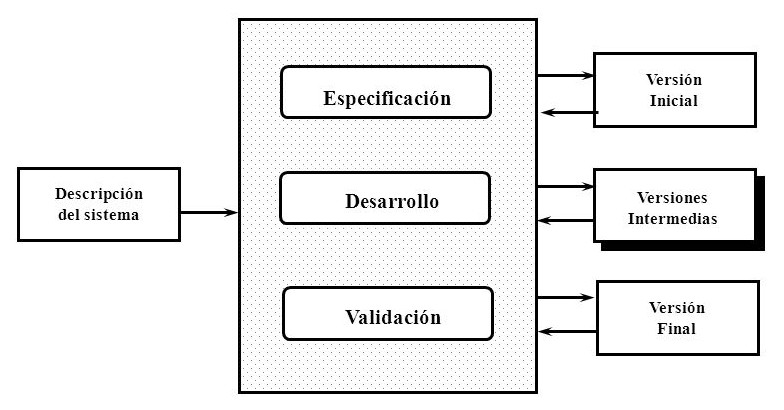
\includegraphics[scale=1, fbox={\fboxrule} 4mm]{images/04-metodo/01-protipado_evolutivo.jpg}
\caption{Prototipado Evolutivo}
\label{fig:prototipado_evolutivo}
\end{figure}

\section{Kanban}
Kanban es una palabra japonesa que se deriva de \textit{kan} (visual) y \textit{ban} tarjeta. Se desarrolló como parte de una estrategia industrial japonesa para conseguir adecuar la producción a la demanda. Consiste en un sistema de visualización por medio de tarjetas de los recursos en procesos de producción.

Según Scrum Manager, una comunidad profesional para la difusión de Scrum, podríamos definir kanban \cite{Pal15} de la siguiente manera:

\begin{tikzpicture}
	\node[shadowBox] {
	El término kanban aplicado a la gestión ágil de proyectos se refiere a técnicas de representación visual de información para mejorar la eficiencia en la ejecución de las tareas de un proyecto.};
\end{tikzpicture}

Kanban se basa en un sistema de producción que dispara el trabajo solo cuando existe capacidad real para procesarlo\cite{Bahi11}. Este disparador está representado por las tarjetas kanban, que están limitadas en número. Cada tarjeta representa un trabajo a realizar durante todo el proceso de desarrollo. Al llegar a la última fase, la tarjeta queda liberada para representar un nuevo trabajo.

Kanban mantiene únicamente tres reglas de funcionamiento, mostrar el proceso, limitar el trabajo en curso y optimizar el flujo de trabajo.

	\subsection{Mostrar el proceso}
	Consiste en la visualización de todo el proceso de desarrollo mediante un tablero físico (o un tablero virtual accesible por todas las partes, como es el caso de \href{https://trello.com/}{Trello}. El objetivo de este tablero es mejorar el entendimiento del proceso de trabajo actual, anticipar los posibles problemas y ayudar a la toma de decisiones resolutivas.
	Los tableros kanban están formados por tres secciones, tal y como podemos ver en la figura \ref{fig:kanban_table_1}, \textit{To Do}, \textit{Doing} y \textit{Done}, que corresponden a la pila de entrada, el \ac{WIP} y la salida. Estas secciones se dividen en columnas representativas de los procesos de trabajo. En la figura \ref{fig:kanban_table_2} podemos ver un tablero típico con la pila de entrada (pending) y el \ac{WIP} (analysis, development, test y deploy).
	
	\begin{figure}[H]
	\centering
	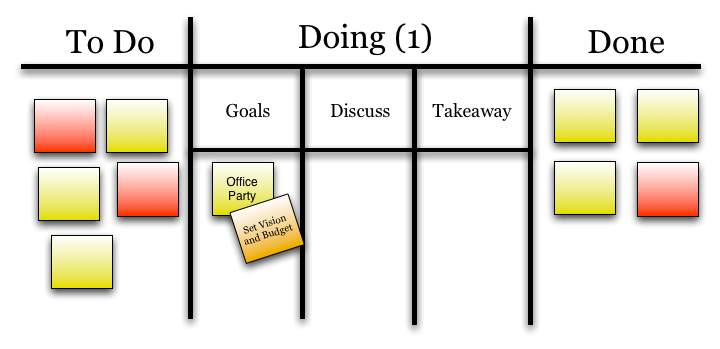
\includegraphics[scale=1, fbox={\fboxrule} 4mm]{images/04-metodo/02-kanban_table_1.png}
	\caption{Secciones tablero kanban}
	\label{fig:kanban_table_1}
	\end{figure}
	
	\begin{figure}[H]
	\centering
	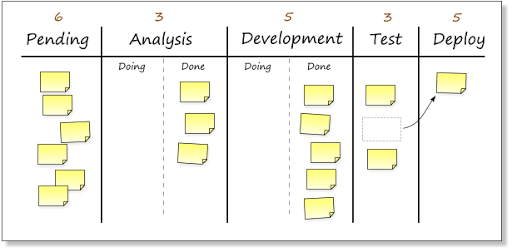
\includegraphics[scale=1, fbox={\fboxrule} 4mm]{images/04-metodo/03-kanban_table_2.png}
	\caption{Columnas tablero kanban}
	\label{fig:kanban_table_2}
	\end{figure}
	
	\subsection{Limitar el trabajo}
	Consiste en limitar la cantidad de ítems o tarjetas que pueden abordarse al mismo tiempo para un proceso definido, es decir, las columnas del tablero. Esta cantidad puede ser visualizada añadiendo el número máximo de tarjetas permitidas a cada columna como un número entre paréntesis al lado del nombre del proceso.
	Esta regla es muy útil para detectar rápidamente los posibles cuellos de botella que puedan producirse. En la imagen \ref{fig:kanban_table_3} podemos observar un desarrollo con un cuello de botella en el proceso \textit{Pruebas}.
	
	\begin{figure}[H]
	\centering
	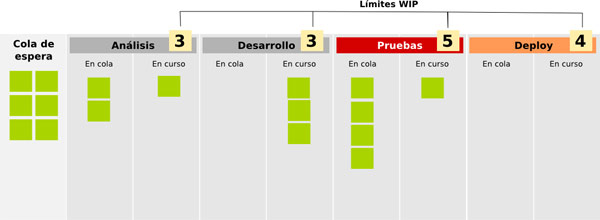
\includegraphics[scale=1, fbox={\fboxrule} 4mm]{images/04-metodo/04-kanban_table_3.jpg}
	\caption{Cuello de botella en kanban}
	\label{fig:kanban_table_3}
	\end{figure}

\section{\acs{TDD}}
	\acf{TDD} es una metodología de desarrollo ágil consistente en escribir primero las pruebas para después implementar el código necesario para pasarlas satisfactoriamente. Según Carlos Blé \cite{Ble10}, podríamos definirlo como:
	
	\begin{tikzpicture}
	\node[shadowBox] {
	\ac{TDD} es una técnica para diseñar software que se centra en tres pilares fundamentales:
	\begin{itemize}[label={$\bullet$},labelindent=\parindent,leftmargin=2cm]
		\item La implementación de las funciones justas que el cliente necesita.
		\item La minimización del número de defectos que llegan a la fase de producción.
		\item La producción de software modular, altamente reutilizable y preparado para el cambio.
	\end{itemize}
	};
\end{tikzpicture}

	\subsection{Algoritmo \ac{TDD}}
	El algoritmo para realizar \ac{TDD} consta únicamente de tres pasos (ver figura \ref{fig:tdd_algorithm}):
	
	\begin{enumerate}
		\item Escribir el test para el requisito a desarrollar elegido
		\item Implementar el código necesario para pasar el test
		\item Refactorizar el código para eliminar duplicidades y mejorarlo.
	\end{enumerate}
	
	\begin{figure}[H]
	\centering
	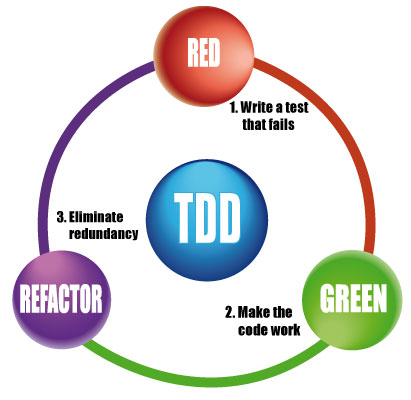
\includegraphics[scale=1, fbox={\fboxrule} 4mm]{images/04-metodo/05-tdd.jpg}
	\caption{Algoritmo TDD}
	\label{fig:tdd_algorithm}
	\end{figure}
	
	\subsection{Ventajas de usar \ac{TDD}}
	Según Kent Beck \cite{Beck04}, creador de TDD, estas son algunas de las principales ventajas de su uso:
	
	\begin{itemize}[label={$\bullet$},labelindent=\parindent,leftmargin=2cm]
		\item La calidad del software aumenta.
		\item Escribir el test antes que el código obliga a escribir el mínimo de funcionalidad necesaria evitando diseños innecesarios.
		\item Los tests son la mejor documentación técnica para consultar qué misión cumple cada parte del código.
	\end{itemize}
	

\section{Marco tecnológico}
En esta sección se incluyen las herramientas y tecnologías utilizadas para el desarrollo del \ac{TFG}.

	\subsection{Herramientas de diseño}
		\subsubsection{Visual Paradigm}
		
		\subsubsection{Gantt Project}
		
		\subsubsection{Moqups}		
	
	\subsection{Herramientas de gestión del proyecto}
		\subsubsection{Git}
		
		\subsubsection{Github}

		\subsubsection{Trello}
	
	\subsection{Herramientas, tecnologías y frameworks para el desarrollo}
		\subsubsection{Ruby}
		
		\subsubsection{Rails}
		
		\subsubsection{Java Android}
		
		\subsubsection{AngularJS}

		\subsubsection{Bootstrap}
		
		\subsubsection{Rspec}
		
		\subsubsection{HTML}
		
		\subsubsection{CSS}
		
		\subsubsection{JSON}
		
		\subsubsection{Sublime Text 3}
		
		\subsubsection{Midori}
	
	\subsection{Herramientas para la gestión de bases de datos}
		\subsubsection{MongoDB}
		
		\subsubsection{RoboMongo}
	
	\subsection{Herramientas documentales}
		\subsubsection{TexMaker}
		
		\subsubsection{GIMP}
		
		\subsubsection{Microsoft Visio}
	
	\subsection{Herramientas de implantación}
		\subsubsection{Heroku}

% Local Variables:
%  coding: utf-8
%  mode: latex
%  mode: flyspell
%  ispell-local-dictionary: "castellano8"
% End:
